\part{Outils pour l'analyse}

\section{Maximum, minimum d'une fonction}\label{maxmin}

\begin{tipblock}
\cmaj{3.04c} L'idée est de proposer une commande pour déterminer, par balayage, le maximum ou le minimum d'une fonction \textit{classique}, sur un intervalle donné.

\smallskip

Le package \ctex{xint} se charge des calculs, et les résultats sont stockés dans des macros personnalisables, pour exploitations ultérieures.

\smallskip

{\small\faBomb} Attention cependant à ne pas travailler sur un intervalle trop grand et/ou de demander une précision trop petite, car les calculs risquent d'être longs\ldots
\end{tipblock}

\begin{PresCodeTexPL}{listing only}
%arguments optionnels = macros de stockage
\DetermineMax[précision]{expression xint}{a}{b}[\tmpmax][\tmpmaxvalx]
\DetermineMin[précision]{expression xint}{a}{b}[\tmpmin][\tmpminvalx]
\end{PresCodeTexPL}

\begin{PresCodePL}{}
\DetermineMax{80*x*exp(-0.2*x)}{3}{10}\tmpmax\ en \tmpmaxvalx
\end{PresCodePL}

\begin{PresCodePL}{}
\DetermineMax[0.1]
	{0.6*cos(4.5*(x-4)+2.1)-1.2*sin(x-4)+0.1*x+0.2}{1}{4}
	[\MonMax]
	[\MonMaxX]
\MonMax\ en \MonMaxX
\end{PresCodePL}

\begin{PresCodePL}{}
\DetermineMin[0.001]
	{log(exp(-x)+1)+0.25*x}{1}{1.2}
	[\MonMin]
	[\MonMinX]
\MonMin\ en \MonMinX
\end{PresCodePL}

\pagebreak

\section{Résolution approchée d'une équation}\label{resolapprox}

\subsection{Idée}

\begin{tipblock}
\cmaj{2.1.4} L'idée est de proposer une commande pour résoudre, de manière approchée, une équation du type $f(x)=k$ sur un intervalle (fermé) donné.

\smallskip

La méthode utilisée est la \textbf{dichotomie}, pour plus de rapidité que la méthode \textit{simple} par balayage.
\end{tipblock}

\begin{PresCodeTexPL}{listing only}
\ResolutionApprochee[clés]{équation}[macro]
\end{PresCodeTexPL}

\begin{PresCodePL}{}
\ResolutionApprochee[Intervalle=0:10]{x**3-2*x**2-x-1=2}%
$x_0 \approx \num[minimum-decimal-digits=2]{\masolutiond}$ par défaut ;\\
$x_0 \approx \num[minimum-decimal-digits=2]{\masolutione}$ par excès ;\\
$x_0 \approx \num[minimum-decimal-digits=2]{\masolutiona}$ arrondi à $10^{-2}$.\\

\hfill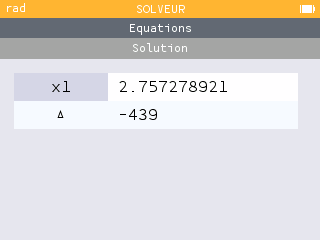
\includegraphics[scale=0.45]{./graphics/pl-solve_a}\hfill~
\end{PresCodePL}

\subsection{Clés et options}

\begin{cautionblock}
Quelques explications sur les \Cle{clés} et sur les arguments :

\begin{itemize}
	\item la clé \Cle{Precision} pour le nombre de chiffres après la virgule de la solution ; \hfill{}défaut \Cle{2}
	\item la clé (obligatoire !) \Cle{Intervalle} qui permet de préciser l'intervalle initial de recherche ;
	\item la clé \Cle{Variable} qui permet de spécifier la variable de l'équation ;\hfill{}défaut \Cle{x}
	\item l'argument \textit{obligatoire} est l'équation, sous la forme $f(\ldots)=k$ (ou $f(\ldots)$ pour $f(\ldots)=0$) ;
	\item l'argument \textit{optionnel} est la base de la \textit{<macro>} qui sert à stocker les valeurs :
	
	\hfill{}défaut \Cle{masolution}
	\begin{itemize}
			\item \ctex{\textbackslash<macro>d} pour la valeur approchée par défaut ;
			\item \ctex{\textbackslash<macro>e} pour la valeur approchée par excès ;
			\item \ctex{\textbackslash<macro>a} pour la valeur approchée.
		\end{itemize}
\end{itemize}
\vspace*{-\baselineskip}\leavevmode
\end{cautionblock}

\begin{PresCodePL}{}
\ResolutionApprochee[Precision=4,Intervalle=0:2]{exp(0.5*x)+x**2-4=0}%
Une valeur approchée, à $10^{-4}$ près, d'une solution de $\text{e}^{0,5x}+x^2-4=0$ sur $\left[0;2\right]$ est $\beta$ avec :
\begin{itemize}
	\item $\beta \approx \num[minimum-decimal-digits=4]{\masolutiond}$ par défaut ;
	\item $\beta \approx \num[minimum-decimal-digits=4]{\masolutione}$ par excès ;
	\item $\beta \approx \num[minimum-decimal-digits=4]{\masolutiona}$.
\end{itemize}
\ResolutionApprochee[Variable=t,Intervalle=-1:2]{3*t*exp(-0.5*t+1)=4}[SolA]%
Une valeur approchée, à $10^{-2}$ près d'une solution de $3t\,\rm{e}^{-0,5t+1}=4$ est $t_1$ avec :
\begin{itemize}
	\item $t_1 \approx \num[minimum-decimal-digits=2]{\SolAd}$ par défaut ;
	\item $t_1 \approx \num[minimum-decimal-digits=2]{\SolAe}$ par excès ;
	\item $t_1 \approx \num[minimum-decimal-digits=2]{\SolAa}$.
\end{itemize}
\ResolutionApprochee[Precision=3,Variable=t,Intervalle=2:10]{3*t*exp(-0.5*t+1)=4}[SolB]
Une valeur approchée, à $10^{-2}$ près d'une solution de $3t\,\text{e}^{-0,5t+1}=4$ est $t_2$ avec :
\begin{itemize}
	\item $t_2 \approx \num[minimum-decimal-digits=2]{\SolBd}$ par défaut ;
	\item $t_2 \approx \num[minimum-decimal-digits=2]{\SolBe}$ par excès ;
	\item $t_2 \approx \num[minimum-decimal-digits=2]{\SolBa}$.
\end{itemize}

\medskip

\hfill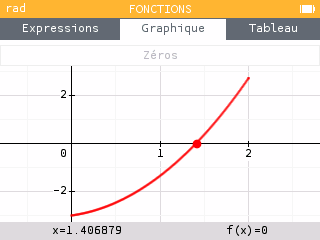
\includegraphics[scale=0.45]{./graphics/pl-solve_b}~~
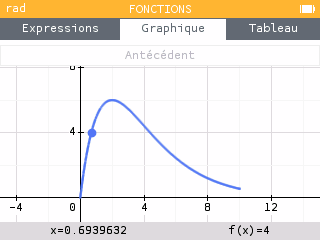
\includegraphics[scale=0.45]{./graphics/pl-solve_c}~~
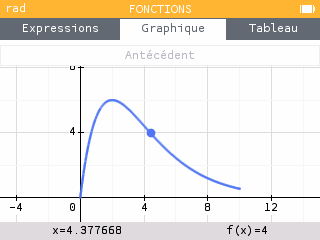
\includegraphics[scale=0.45]{./graphics/pl-solve_d}\hfill~
\end{PresCodePL}

\newpage

\section{Présentation d'une solution d'équation par balayage}\label{solutiontvi}

\subsection{Idée}

\begin{tipblock}
\cmaj{2.0.4} L'idée est de présenter l'obtention d'une solution approchée d'équation par balayage, dans le cadre du TVI par exemple. Les calculs et tests sont effectués grâce au package \ctex{xinttools}, et le formatage par \ctex{tabularray} et \ctex{sinuitx}.
\end{tipblock}

\begin{warningblock}
Le code ne trouve pas la solution, il met \textit{juste} en forme mais effectue quand même les calculs d'images et les tests.
\end{warningblock}

\begin{PresCodeTexPL}{listing only}
\SolutionTVI[options]{fonction}{valeur}
\end{PresCodeTexPL}

\subsection{Clés et arguments}

\begin{cautionblock}
Plusieurs \Cle{Clés} sont disponibles pour cette commande, relative à une équation du type $f(x)=k$ :

\begin{itemize}
	\item la clé \Cle{NomFct} qui permet de spécifier le nom de la fonction ;\hfill{}défaut \Cle{f}
	\item la clé \Cle{NomSol} qui permet de spécifier le nom de la fonction ;\hfill{}défaut \Cle{\textbackslash{}alpha}
	\item les clés \Cle{va} et \Cle{vb} qui sont les bornes inférieure et supérieure de l'encadrement ;
	\item la clé \Cle{Precision} qui est la précision des calculs pour les images ;\hfill{}défaut \Cle{2}
	\item la clé \Cle{Stretch} qui permet d'espacer les lignes ;\hfill{}défaut \Cle{1.15}
	\item les booléens \Cle{Balayage} ou \Cle{Calculatrice} pour afficher un texte en amont ;\hfill{}défaut \Cle{false}
	%\item le booléen \Cle{Simple} pour une présentation plus \textit{neutre} ;\hfill{}défaut \Cle{false}
	\item le booléen \Cle{Majuscule} qui affiche le texte avant, avec une majuscule au début.\hfill{}défaut \Cle{true}
\end{itemize}

\smallskip

Le premier argument \textit{obligatoire} est la fonction, en syntaxe \ctex{xint} et avec comme variable $x$, et le second la valeur de $k$.
\end{cautionblock}

\begin{PresCodePL}{}
Pour $f(x)=0$ avec $f(x)=x^2-2$. On obtient \SolutionTVI[va=1.414,vb=1.415,Precision=3]{x**2-2}{0}.
\end{PresCodePL}

\begin{PresCodePL}{}
Avec $\varphi(t)=3t\,\rm{e}^{-0,5t+1}=5$,
\SolutionTVI[Majuscule=false,Calculatrice,va=1.02,vb=1.03,NomFct=\varphi]
	{3*x*exp(-0.5*x+1)}{5}
\end{PresCodePL}

\begin{PresCodePL}{}
On s'intéresse à $g(x)=\num{1,5}$ avec $g(x)=\ln(x)$.\\
\SolutionTVI%
	[Balayage,Stretch=1.5,va=4.48,vb=4.49,NomFct=g,Precision=4,NomSol={x_0}]{log(x)}{1.5}.
\end{PresCodePL}

\subsection{Interaction avec la commande de résolution approchée}

\begin{tipblock}
\cmaj{2.1.4} L'idée est de récupérer les valeurs par défaut et par excès pour le TVI grâce à la commande \ctex{\textbackslash ResolutionApprochee}.
\end{tipblock}

\begin{PresCodePL}{}
On s'intéresse à $g(x)=\num{1,5}$ avec $g(x)=\ln(x)$ sur l'intervalle $\left[3;5\right]$.

\ResolutionApprochee[Intervalle=3:5]{log(x)=1.5}[SolLn]
\SolutionTVI%
	[Balayage,Stretch=1.5,va={\SolLnd},vb={\SolLne},
	NomFct=g,Precision=4,NomSol={x_0}]{log(x)}{1.5}.
\end{PresCodePL}

\begin{noteblock}
À terme, peut-être que la commande \ctex{\textbackslash ResolutionApprochee} sera intégrée dans la commande \ctex{\textbackslash SolutionTVI} afin d'automatiser encore plus le procédé.
\end{noteblock}

\newpage

\section{Suites récurrentes simples}\label{calcrecurr}

\subsection{Idées}

\begin{tipblock}
\cmaj{2.0.3} L'idée est de proposer des commandes pour effectuer des calculs avec des suites récurrentes du type $u_{n+1}=f\big(u_n\big)$ :

\begin{itemize}
	\item calcul de termes avec possibilité d'arrondir ;
	\item présentation de la conclusion de la recherche d'un seuil du type $u_n > S$ ou $u_n < S$.
\end{itemize}
\vspace*{-\baselineskip}\leavevmode
\end{tipblock}

\begin{warningblock}
\cmaj{2.1.0} Le code pour le seuil \textbf{trouve} également le rang cherché, il met en forme et effectue les calculs d'images.

\smallskip

\cmaj{2.0.5} Le choix a été fait de faire les calculs en mode \ctex{float} pour éviter les dépassements de capacité de \ctex{xint} liés aux boucles\ldots
\end{warningblock}

\begin{PresCodeTexPL}{listing only}
%commande pour calculer et formater
\CalculTermeRecurrence[options]{fonction associée}

%mise en forme de la conclusion d'un seuil
\SolutionSeuil[options]{fonction associée}{seuil}
\end{PresCodeTexPL}

\subsection{Clés et arguments}

\begin{cautionblock}
Plusieurs \Cle{Clés} sont disponibles pour la commande du calcul d'un terme :

\begin{itemize}
	\item la clé \Cle{No} qui est le rang initial de la suite ;
	\item la clé \Cle{UNo} qui est le terme initial de la suite ;
	\item la clé \Cle{Precision} qui précise l'arrondi éventuel ;\hfill{}défaut \Cle{3}
	\item la clé \Cle{N} qui est l'indice du terme à calculer.
\end{itemize}

\smallskip

L'argument \textit{obligatoire} est la fonction associée à la suite, en syntaxe \ctex{xint} et avec comme variable $x$.
\end{cautionblock}

\begin{PresCodeTexPL}{listing only}
Avec $\begin{dcases} u_0 = 50 \\ u_{n+1}=\dfrac{1}{u_n+2} \end{dcases}$.

On obtient $u_{10} \approx \CalculTermeRecurrence[No=0,UNo=50,N=10]{1/(x+2)}$.

On obtient $u_{15} \approx \CalculTermeRecurrence[Precision=4,No=0,UNo=50,N=15]{1/(x+2)}$.

On obtient $u_{20} \approx \CalculTermeRecurrence[Precision=6,No=0,UNo=50,N=20]{1/(x+2)}$.
\end{PresCodeTexPL}

\begin{PresCodeSortiePL}{text only}
Avec $u_0 = 50$ et $u_{n+1}=\dfrac{1}{u_n+2}$.

\smallskip

On obtient $u_{10} \approx \CalculTermeRecurrence[No=0,UNo=50,N=10]{1/(x+2)}$ \hfill~sortie par défaut.

\smallskip

On obtient $u_{15} \approx \CalculTermeRecurrence[Precision=4,No=0,UNo=50,N=15]{1/(x+2)}$  \hfill~avec choix de la précision à $10^{-4}$.

\smallskip

On obtient $u_{20} \approx \CalculTermeRecurrence[Precision=6,No=0,UNo=50,N=20]{1/(x+2)}$ \hfill~avec choix de la précision à $10^{-6}$.
\end{PresCodeSortiePL}

\begin{cautionblock}
Plusieurs \Cle{Clés} sont disponibles pour la commande du seuil :

\begin{itemize}
	\item la clé \Cle{NomSuite} qui est le nom de la suite ;\hfill~défaut \Cle{u}
	\item la clé \Cle{No} qui est le rang initial de la suite ;
	\item la clé \Cle{UNo} qui est le terme initial de la suite ;
	%\item la clé \Cle{SolN} qui est la valeur de l'indice cherché ;
	\item la clé \Cle{Precision} qui précise l'arrondi éventuel ;\hfill{}défaut \Cle{2}
	\item la clé \Cle{Stretch} qui permet d'espacer les lignes ;\hfill{}défaut \Cle{1.15}
	\item les booléens \Cle{Balayage} ou \Cle{Calculatrice} pour afficher un texte en amont ;\hfill{}défaut \Cle{false}
	\item le booléen \Cle{Simple} pour une présentation plus \textit{neutre} ;\hfill{}défaut \Cle{false}
	\item le booléen \Cle{Majuscule} qui affiche le texte avant, avec une majuscule au début ;\hfill{}défaut \Cle{true}
	\item les booléens \Cle{Exact} et \Cle{ExactB} qui affichent \ctex{=} au lieu de \ctex{\textbackslash approx} ;\hfill{}défaut \Cle{false}
	\item le booléen \Cle{Conclusion} pour afficher la conclusion ou non ;\hfill{}défaut \Cle{true}
	\item la clé \Cle{Sens} parmi \Cle{< / > / <= / >=} pour indiquer le type de seuil.\hfill{}défaut \Cle{>}
\end{itemize}

\smallskip

Le premier argument \textit{obligatoire} est la fonction associée à la suite, en syntaxe \ctex{xint} et avec comme variable $x$, et le second est le seuil à dépasser.
\end{cautionblock}

\begin{PresCodePL}{}
Avec $\begin{dcases} u_1 = 2 \\ u_{n+1}=1+\dfrac{1+u_n^2}{1+u_n} \end{dcases}$,
on cherche $n$ tel que $u_n > 5$.\\
\SolutionSeuil[Balayage,No=1,UNo=2]{1+(1+x**2)/(1+x)}{5}. \SolutionSeuil[Calculatrice,Precision=4,No=1,UNo=2,Conclusion=false]%
{1+(1+x**2)/(1+x)}{5}.
\end{PresCodePL}

\subsection{Exemple d'utilisation}

\begin{PresCodePL}{}
Avec $\begin{dcases} u_1 = 2 \\ u_{n+1}=1+\dfrac{1+u_n^2}{1+u_n} \end{dcases}$,
on obtient le tableau de valeurs suivant : 
\begin{tabular}{c|c}
	$n$ & $u_n$ \\ \hline
	1 & 2 \\
	\xintFor* #1 in {\xintSeq{2}{7}} \do {#1 & \CalculTermeRecurrence[No=1,UNo=2,N=#1]{1+(1+x**2)/(1+x)} \\}
\end{tabular}\\

\SolutionSeuil[Precision=4,No=1,UNo=2,Simple]{1+(1+x**2)/(1+x)}{10} (Ainsi $u_n > 10$ à partir de $n=\the\CompteurSeuil$)
\end{PresCodePL}

\newpage

\section{Valeur approchée d'une intégrale}\label{calcintegr}

\subsection{Idée}

\begin{tipblock}
\cmaj{2.6.1} L'idée est de proposer plusieurs approximations pour le calcul d'une intégrale, en utilisant :
\begin{itemize}
	\item une méthode des rectangles (Gauche, Droite ou Milieu) ;
	\item la méthode des trapèzes ;
	\item la méthode de Simpson.
\end{itemize}
\vspace*{-\baselineskip}\leavevmode
\end{tipblock}

\begin{warningblock}
Il s'agit de valeurs approchées, mais la méthode de Simpson donne des valeurs satisfaisantes !

Les méthodes \textit{Rectangles} ou \textit{Trapèzes} seront plutôt utiles pour des résultats obtenus par algorithme par exemple.
\end{warningblock}

\begin{PresCodeTexPL}{listing only}
\IntegraleApprochee[clés]{fonction}{a}{b}
\end{PresCodeTexPL}

\subsection{Clés et arguments}

\begin{cautionblock}
Plusieurs \Cle{Clés} sont disponibles pour la commande de calcul :

\begin{itemize}
	\item le booléen \Cle{ResultatBrut} qui donne le résultat obtenu grâce à \ctex{xint} ; \hfill~défaut : \Cle{false}
	\item la clé \Cle{Methode}, parmi \Cle{RectanglesGauche / RectanglesDroite / RectanglesMilieu / Trapezes / Simpson} pour spécifier la méthode utilisée ;
	
	\hfill~défaut : \Cle{Simpson}
	\item la clé \Cle{NbSubDiv} précise le nombre de subdivisions pour le calcul ; \hfill~défaut : \Cle{10}
	\item le booléen \Cle{AffFormule} qui affiche au préalable l'intégrale ;\hfill{}défaut \Cle{false}
	\item la clé \Cle{Expr} qui indique ce qui doit être affiché dans l'intégrale ; \hfill{}défaut \Cle{f(x)}
	\item la clé \Cle{Signe} qui indique le signe à afficher entre l'intégrale et le résultat ; \hfill{}défaut \Cle{\textbackslash approx}
	\item la clé \Cle{Variables} qui indique la variable à afficher dans le $\text{d}x$. \hfill{}défaut \Cle{x}
\end{itemize}

\smallskip

Concernant les arguments obligatoires :

\begin{itemize}
	\item le premier est la fonction à intégrer, en langage \ctex{xint}, avec comme variable $x$ ;
	\item les deux autres arguments sont les bornes de l'intégrale.
\end{itemize}

À noter que la commande, hormis dans sa version \Cle{ResultatBrut}, est à insérer de préférence dans un mode mathématique.
\end{cautionblock}

\begin{PresCodePL}{}
On s'intéresse à $\displaystyle\int_4^{10} f(x) \,\text{d}x$ avec $f(x)=\sqrt{x}$ :\\
\begin{itemize}[itemsep=6pt,leftmargin=4cm]
	\item[\texttt{sortie par défaut} :] \IntegraleApprochee{sqrt(x)}{4}{10}
	\item[\texttt{résultat brut} :] \IntegraleApprochee[ResultatBrut]{sqrt(x)}{4}{10}
	\item[\texttt{résultat formaté} :] $\displaystyle\IntegraleApprochee[NbSubDiv=100,AffFormule,Precision=5,Expr={\sqrt{x}}]%
		{sqrt(x)}{4}{10}$
\end{itemize}
\end{PresCodePL}

\subsection{Exemples}

\begin{PresCodeTexPL}{listing only}
%tableau
\IntegraleApprochee[NbSubDiv=10,ResultatBrut]{sqrt(x)}{4}{10}
\IntegraleApprochee[NbSubDiv=10,Methode=RectanglesGauche,ResultatBrut]{sqrt(x)}{4}{10}
\IntegraleApprochee[NbSubDiv=10,Methode=RectanglesDroite,ResultatBrut]{sqrt(x)}{4}{10}
\IntegraleApprochee[NbSubDiv=10,Methode=RectanglesMilieu,ResultatBrut]{sqrt(x)}{4}{10}
\IntegraleApprochee[NbSubDiv=10,Methode=Trapezes,ResultatBrut]{sqrt(x)}{4}{10}
$\displaystyle\IntegraleApprochee[NbSubDiv=10,AffFormule,Expr={\sqrt{x}}]{sqrt(x)}{4}{10}$
\end{PresCodeTexPL}

\begin{PresCodeSortiePL}{text only}
\begin{tblr}[B]{hlines,vlines,colspec={Q[5cm,m,l]Q[5cm,m,l]},row{1}={halign=c,font=\bfseries\sffamily,bg=lightgray}}
	Méthode utilisée & Valeur brute obtenue \\
	\SetCell[c=2]{c} $f(x)=\sqrt{x}$ et $n=10$ ; $\displaystyle\int_4^{10} f(x) \,\text{d}x$ & \\
	Simpson & $\IntegraleApprochee[NbSubDiv=10,Methode=Simpson,ResultatBrut]{sqrt(x)}{4}{10}$ \\
	rectangles Gauche & $\IntegraleApprochee[NbSubDiv=10,Methode=RectanglesGauche,ResultatBrut]{sqrt(x)}{4}{10}$ \\
	rectangles Droite & $\IntegraleApprochee[NbSubDiv=10,Methode=RectanglesDroite,ResultatBrut]{sqrt(x)}{4}{10}$ \\
	rectangles Milieu & $\IntegraleApprochee[NbSubDiv=10,Methode=RectanglesMilieu,ResultatBrut]{sqrt(x)}{4}{10}$ \\
	trapèzes & $\IntegraleApprochee[NbSubDiv=10,Methode=Trapezes,ResultatBrut]{sqrt(x)}{4}{10}$ \\
	\SetCell[c=2]{c} $\displaystyle\IntegraleApprochee[NbSubDiv=10,AffFormule,Expr={\sqrt{x}}]{sqrt(x)}{4}{10}$ & \\
\end{tblr}~~
\includegraphics[height=3cm]{integr_nwks_a}
\end{PresCodeSortiePL}

\begin{PresCodeTexPL}{listing only}
%tableau
\IntegraleApprochee[NbSubDiv=100,Methode=Simpson,ResultatBrut]{80*x*exp(-0.2*x)}{1}{20}
\IntegraleApprochee[NbSubDiv=100,Methode=RectanglesGauche,ResultatBrut]{80*x*exp(-0.2*x)}{1}{20}
\IntegraleApprochee[NbSubDiv=100,Methode=RectanglesDroite,ResultatBrut]{80*x*exp(-0.2*x)}{1}{20}
\IntegraleApprochee[NbSubDiv=100,Methode=RectanglesMilieu,ResultatBrut]{80*x*exp(-0.2*x)}{1}{20}
\IntegraleApprochee[NbSubDiv=100,Methode=Trapezes,ResultatBrut]{80*x*exp(-0.2*x)}{1}{20}
$\displaystyle\IntegraleApprochee[NbSubDiv=100,AffFormule,Expr={80x\,\text{e}^{-0,2x}}]%
	{80*x*exp(-0.2*x)}{1}{20}$
\end{PresCodeTexPL}

\begin{PresCodeSortiePL}{text only}
\begin{tblr}[B]{hlines,vlines,colspec={Q[5cm,m,l]Q[5cm,m,l]},row{1}={halign=c,font=\bfseries\sffamily,bg=lightgray}}
	Méthode utilisée & Valeur brute obtenue \\
	\SetCell[c=2]{c} $f(x)=80x\,\text{e}^{-0,2x}$ et $n=100$ ; $\displaystyle\int_1^{20} f(x) \,\text{d}x$ & \\
	Simpson & $\IntegraleApprochee[NbSubDiv=100,Methode=Simpson,ResultatBrut]{80*x*exp(-0.2*x)}{1}{20}$ \\
	rectangles Gauche & $\IntegraleApprochee[NbSubDiv=100,Methode=RectanglesGauche,ResultatBrut]{80*x*exp(-0.2*x)}{1}{20}$ \\
	rectangles Droite & $\IntegraleApprochee[NbSubDiv=100,Methode=RectanglesDroite,ResultatBrut]{80*x*exp(-0.2*x)}{1}{20}$ \\
	rectangles Milieu & $\IntegraleApprochee[NbSubDiv=100,Methode=RectanglesMilieu,ResultatBrut]{80*x*exp(-0.2*x)}{1}{20}$ \\
	trapèzes & $\IntegraleApprochee[NbSubDiv=100,Methode=Trapezes,ResultatBrut]{80*x*exp(-0.2*x)}{1}{20}$ \\
	\SetCell[c=2]{c} $\displaystyle\IntegraleApprochee[NbSubDiv=100,AffFormule,Expr={80x\,\text{e}^{-0,2x}}]{80*x*exp(-0.2*x)}{1}{20}$ & \\
\end{tblr}~~
\includegraphics[height=3cm]{integr_nwks_b}
\end{PresCodeSortiePL}

\subsection{Commande simplifiée}\label{calculintegrale}

\begin{tipblock}
\cmaj{3.04a} À noter qu'il existe une commande, simplifiée, pour le calcul de la valeur approchée d'une intégrale :
\begin{itemize}
	\item la méthode utilisée est la méthode de Simpson ;
	\item il n'existe pas de \Cle{clés} pour cette commande.
\end{itemize}
\vspace*{-\baselineskip}\leavevmode
\end{tipblock}

\begin{PresCodeTexPL}{listing only}
\CalcIntegrale(*)[prec]<nb subdiv>{expr version xint}{binf}{bsup}
\end{PresCodeTexPL}

\begin{cautionblock}
La version étoilée force l'affichage avec \ctex{sinuitx}.

L'argument optionnel, et entre \ctex{[...]}, est la précision éventuelle souhaitée (résultat brut sinon).

L'argument optionnel, et entre \ctex{<...>}, est le nombre de subdivisions, qui permet de gagner en précision.

Les trois arguments obligatoires sont quant à eux :
\begin{itemize}
	\item l'expression de la fonction, en langage \ctex{xint} ;
	\item les bornes de l'intégrale.
\end{itemize}
\vspace*{-\baselineskip}\leavevmode
\end{cautionblock}

\begin{PresCodePL}{}
$\displaystyle\int_1^{20} 80x\e^{-0,2x} \,\text{d}x \approx
\CalcIntegrale{80*x*exp(-0.2*x)}{1}{20}$
\end{PresCodePL}

\begin{PresCodePL}{}
$\displaystyle\int_1^{20} 80x\e^{-0,2x} \,\text{d}x \approx
\CalcIntegrale*{80*x*exp(-0.2*x)}{1}{20}$
\end{PresCodePL}

\begin{PresCodePL}{}
$\displaystyle\int_1^{20} 80x\e^{-0,2x} \,\text{d}x \approx
\CalcIntegrale*[3]{80*x*exp(-0.2*x)}{1}{20}$
\end{PresCodePL}

\begin{tipblock}
\cmaj{3.04a} On peut également utiliser la commande, avec exactement le même fonctionnement, pour déterminer une estimation d'une valeur moyenne par intégrale.
\end{tipblock}

\begin{PresCodeTexPL}{listing only}
\ValeurMoyenneIntg(*)[prec]<nb subdiv>{expr version xint}{binf}{bsup}
\end{PresCodeTexPL}

\begin{PresCodePL}{}
$\displaystyle\dfrac{1}{20-1}\int_1^{20} 80x\e^{-0,2x} \,\text{d}x \approx
\ValeurMoyenneIntg*[3]<100>{80*x*exp(-0.2*x)}{1}{20}$
\end{PresCodePL}

\newpage

\section{Forme canonique, fonction homographique}\label{canonhomo}

\subsection{Idée}

\begin{tipblock}
\cmaj{3.03a} L'idée est de proposer des commandes pour :
\begin{itemize}
	\item mettre un trinôme sous forme canonique $ax^2+bx+c = a(x-\alpha)^2+\beta$ ($a \neq 0$) ;
	\item décomposer une fonction homographique $\frac{ax+b}{cx+d}=A+\frac{C}{x-\alpha}$ ($c \neq 0$).
\end{itemize}
\vspace*{-\baselineskip}\leavevmode
\end{tipblock}

\begin{PresCodeTexPL}{listing only}
\FormeCanonique(*)[option]{a}{b}{c}
\end{PresCodeTexPL}

\begin{PresCodeTexPL}{listing only}
\FonctionHomographique(*)[option]{a}{b}{c}{d}
\end{PresCodeTexPL}

\subsection{Forme canonique}

\begin{tipblock}
La version étoilée force l'affichage (si besoin) du signe \og $-$ \fg, sous la forme $a(x-\alpha)^2+\beta$ ; et le code se charge de gérer les cas particuliers ($|a|=1$, $\alpha=0$, $\beta=0$).

\smallskip

Le code devrait fonctionner correctement avec des entiers et/ou des décimaux, mais les résultats affichés le seront toujours sous forme fractionnaire (par défaut, l'argument optionnel vaut \Cle{[d]} pour formater en \ctex{\textbackslash displaystyle}, mais on, peut utiliser \Cle{[t/n/dec]}).
\end{tipblock}

\begin{PresCodePL}{}
$2x^2+4x-6 = \FormeCanonique{2}{4}{-6} = \FormeCanonique*{2}{4}{-6}$
\end{PresCodePL}

\begin{PresCodePL}{}
$-x^2+4x-6 = \FormeCanonique{-1}{4}{-6}$
\end{PresCodePL}

\begin{PresCodePL}{}
$x^2+3x+7 = \FormeCanonique{1}{3}{7} = \FormeCanonique*{1}{3}{7}$
\end{PresCodePL}

\begin{PresCodePL}{}
$3x^2-7x = \FormeCanonique{3}{-7}{0} = \FormeCanonique[t]{3}{-7}{0}$
\end{PresCodePL}

\begin{PresCodePL}{}
$3x^2-7 = \FormeCanonique{3}{0}{-7}$
\end{PresCodePL}

\begin{PresCodePL}{}
$x^2+2x+1 = \FormeCanonique{1}{2}{1}$
\end{PresCodePL}

\begin{PresCodePL}{}
$1,5x^2-7,25x-14 = \FormeCanonique{1.5}{-7.25}{-14}$
\end{PresCodePL}

\subsection{Fonction homographique}

\begin{tipblock}
La version étoilée force l'affichage (si besoin) du signe \og $-$ \fg{} au dénominateur, sous la forme $x-\alpha$ ; et le code se charge de gérer les cas particuliers ($|A|=1$, $\alpha=0$, $B=0$).

\smallskip

Le code devrait fonctionner correctement avec des entiers et/ou des décimaux, mais les résultats affichés le seront toujours sous forme fractionnaire :

\begin{itemize}
	\item le coefficient $A$ est toujours en mode \ctex{dfrac}, tout comme la fraction \textit{principale} ;
	\item les coefficients $B$ et $\alpha$ sont par défaut en \ctex{tfrac}, mais l'argument optionnel peut valoir \Cle{[d/t/n/dec]}.
\end{itemize}
\vspace*{-\baselineskip}\leavevmode
\end{tipblock}

\begin{PresCodePL}{}
$\dfrac{2x-11}{3x-6} = \FonctionHomographique{2}{-11}{3}{-6}$
\end{PresCodePL}

\begin{PresCodePL}{}
$\dfrac{11}{3x+6} = \FonctionHomographique{0}{11}{3}{6} = \FonctionHomographique*{0}{11}{3}{6}$
\end{PresCodePL}

\begin{PresCodePL}{}
$\dfrac{2x+5}{7x-19} = \FonctionHomographique{2}{5}{7}{-19}$
\end{PresCodePL}

\begin{PresCodePL}{}
$\dfrac{2x+5}{4x} = \FonctionHomographique{2}{5}{4}{0}$
\end{PresCodePL}

\begin{PresCodePL}{}
$\dfrac{-x+7}{7x-5} = \FonctionHomographique{-1}{7}{7}{-5} = \FonctionHomographique*{-1}{7}{7}{-5}$
\end{PresCodePL}